% ============================================================
% Illustration: Ben-David bound components d_{HdH} and lambda*
% and how SFM / few-shot / mixup act on them.
% Compile standalone -> fig_bendavid.pdf, place in figure-q1/.
% Answers reviewer: "a graphical visualization of d_{HdH} and lambda*".
% ============================================================
\documentclass[tikz,border=6pt]{standalone}
\usepackage{helvet}\renewcommand{\familydefault}{\sfdefault}
\usepackage{amsmath}
\usepackage{tikz}
\usetikzlibrary{arrows.meta,positioning,backgrounds,fit,decorations.pathreplacing}
\begin{document}
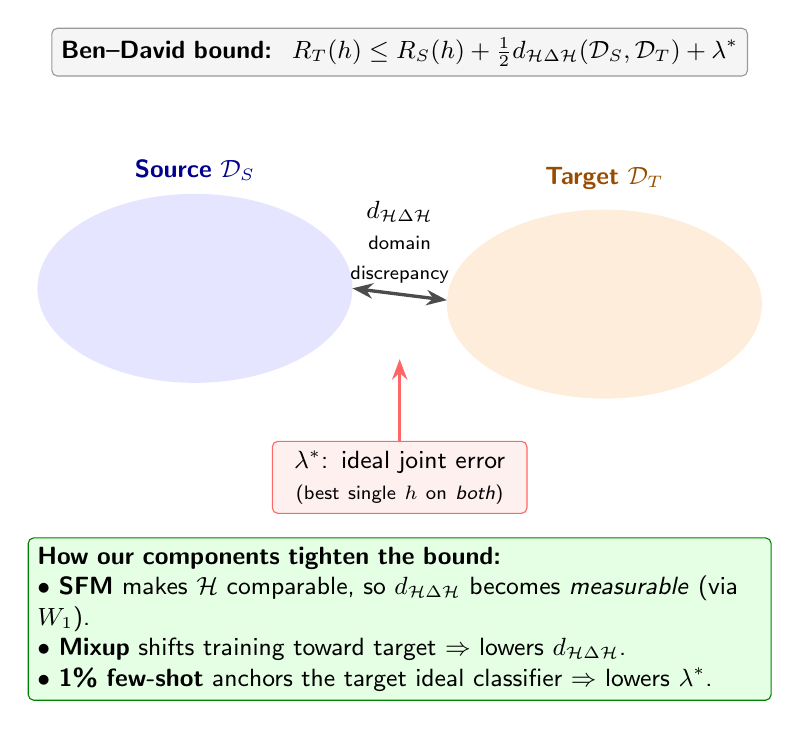
\begin{tikzpicture}[font=\small,>={Stealth[length=2.6mm]}]

% Two feature clouds: source (S) and target (T)
\begin{scope}
  \fill[blue!10,rounded corners=10pt] (0,0) ellipse (2.0 and 1.2);
  \node[blue!55!black] at (0,1.5) {\textbf{Source} $\mathcal{D}_S$};
  \fill[orange!14,rounded corners=10pt] (5.2,-0.2) ellipse (2.0 and 1.2);
  \node[orange!60!black] at (5.2,1.4) {\textbf{Target} $\mathcal{D}_T$};
\end{scope}

% Discrepancy arrow between the clouds
\draw[<->,line width=1.2pt,draw=black!70] (2.0,0) -- (3.2,-0.15)
  node[midway,above,align=center]{$d_{\mathcal{H}\Delta\mathcal{H}}$\\\scriptsize domain\\\scriptsize discrepancy};

% Ideal joint hypothesis error lambda*
\node[draw=red!60,fill=red!6,rounded corners=2pt,align=center,text width=30mm]
  (lam) at (2.6,-2.4)
  {$\lambda^\ast$: ideal joint error\\\scriptsize (best single $h$ on \emph{both})};
\draw[->,red!60,line width=0.9pt] (lam.north) -- (2.6,-0.9);

% The bound
\node[draw=black!40,fill=black!4,rounded corners=2pt,align=center,text width=86mm]
  (bound) at (2.6,3.0)
  {\textbf{Ben--David bound:}\;
   $R_T(h)\le R_S(h)+\tfrac12 d_{\mathcal{H}\Delta\mathcal{H}}(\mathcal{D}_S,\mathcal{D}_T)+\lambda^\ast$};

% How each method acts
\node[draw=green!50!black,fill=green!10,rounded corners=2pt,align=left,
      text width=92mm] (act) at (2.6,-4.2)
  {\textbf{How our components tighten the bound:}\\
   $\bullet$ \textbf{SFM} makes $\mathcal{H}$ comparable, so
     $d_{\mathcal{H}\Delta\mathcal{H}}$ becomes \emph{measurable} (via $W_1$).\\
   $\bullet$ \textbf{Mixup} shifts training toward target $\Rightarrow$ lowers
     $d_{\mathcal{H}\Delta\mathcal{H}}$.\\
   $\bullet$ \textbf{1\% few-shot} anchors the target ideal classifier
     $\Rightarrow$ lowers $\lambda^\ast$.};

\end{tikzpicture}
\end{document}
